% Overall overview of the adopted user testing procedure
\section{User Testing}

\subsection{Generalities}
The core purpose of user testing (UT) is to assess the usability properties of a system by observing how the system is used by users that are representative of real end users. 
It is a form of empirical research that aims to understand the relationship between humans and technology, learning how humans interact with a designed system through observed phenomena. 
Users are assigned pre-defined tasks to complete using the system and are then observed, recorded and finally analysed. 
Through user testing we can uncover actual difficulties that users will face, ones perhaps overlooked during the initial design of the system.

\subsection{Design}
The user testing procedure was designed to give probable users tasks that they would likely need to use the UNICEF website for. 
Moreover, as user testing was performed after the inspection phase of the website, the tasks were modeled to investigate further more issues that were previously found. 
The user profile used for recruiting users was aimed at an age range of 20 to 35 as the average age of UNICEF volunteers is reported to around 30. 
Due to this age range’s familiarity with websites and technology in general, the tasks we designed to push their abilities.
After the initial inspection, it was discussed and agreed that the main actions a target user would take on this site are: 

\begin{enumerate}
    \item Donating money
    \item Searching for information
    \item Volunteering with the association
    \item Find contact information
    \item Find the charity’s social media accounts
\end{enumerate}

With each of these actions the quality of the site is not only tested by achieving the desired outcome for each task but also with what ease and efficiency can the user complete each action. 
With each task the user is provided brief context and motivation for the action he or she needs to preform. 
The tasks used for the UT phase are listed below.

\begin{itemize}
    % Task A
    \item [\textbf{A}] You would like to support UNICEF in their work.
    Make a once off donation of 10€ to the charity.\\
    \textbf{\color{unicefRed}{Warning}} : Interrupt this task before confirming payment.

    \item [] \textbf{Time Limit}\\
    3 minutes

    \item [] \textbf{Motivation}\\
    As UNICEF is a charity organisation, a primary goal of their website is to fundraise money. 
    For this reason the action of donation is essential to the success of the website. 

    \newpage
    % Task B
    \item [\textbf{B}] Your manager at work has a letter that must be sent to the ethic’s office of UNICEF.
    Find the appropriate postal address that this letter should be sent to.

    \item [] \textbf{Time Limit}\\
    3 minutes and 30 seconds

    \item [] \textbf{Motivation}\\
    A primary action on a website of this kind is finding relevant contact information.
    After inspecting the website, we chose to ask for the Ethic’s Office postal address specifically as it’s location is not obvious, and so would be a greater test of our technologically apt test group. 

    % Task C
    \item [\textbf{C}] From what you have read on the UNICEF website you are very interested in their work and you would like to be kept up to date with any news from the organisation.
    Find a way to subscribe to new information or updates from UNICEF.

    \item [] \textbf{Time Limit}\\
    3 minutes and 30 seconds

    \item [] \textbf{Motivation}\\
    Getting users to subscribe to information updates is a useful tool for organisations such as UNICEF.

    % Task D
    \item [\textbf{D}] You are interested in working with UNICEF either as an intern or as a volunteer. 
    Find what opportunities are available.

    \item [] \textbf{Time Limit}\\
    3 minutes

    \item [] \textbf{Motivation}\\
    For a charity as large as UNICEF, finding new volunteers and employees is essential.
    We were also interested to see how users felt navigating these sections due to the large amount of information available.

    % Task E
    \item [\textbf{E}] For a university project, you have been asked to write about the impact of charity work on Women’s Rights in Africa. 
    You decide to do some research on the UNICEF website.
    Find out some information on the work the organisation does to help women in Africa. 

    \item [] \textbf{Time Limit}\\
    3 minutes and 30 seconds

    \item [] \textbf{Motivation}\\
    As already mentioned, a primary use of the website is for users to gather information on social issues and the work UNICEF does to help them.
    The task specified the information that needed to be found in order to see would users use the search feature or other methods.
    
    \newpage
    % Task F
    \item [\textbf{F}] You have recently become a parent. 
    Find the area of the website with the relevant information about this topic and sign up.

    \item [] \textbf{Time Limit}\\
    4 minutes and 15 seconds

    \item [] \textbf{Motivation}\\
    This task was chosen due to the action needing to be performed only being possible in one specific location.
    
\end{itemize}

\newpage
\subsection{Execution}
The testing procedure was carried out as uniform as possible across all users, with the exception of two users who tested the mobile version of the website. 
Due to logical constraints, seven users were tested remotely. 
First, users were given an explanation of the tests with their guidelines and rules.  
Then they were given a Google form to fill in with their personal data (such as age, highest education level and some general information about their background) and to collect the time spent on each task. 
The purpose of collecting this information is that it could later be used to explain deviations in users' success with tasks.

\begin{figure}[htp!]
    \centering
    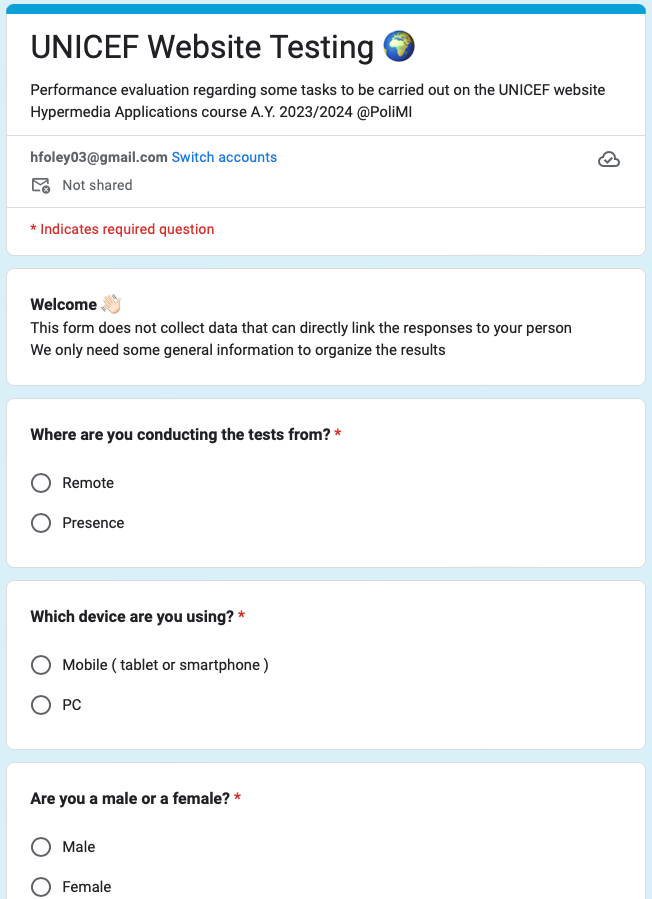
\includegraphics[scale=0.4]{Resources/Harry/GoogleForm.png}
    \caption{Section of the Google Form used to conduct user testing}
\end{figure}

It was decided to provide minimal help to users during the test in order to simulate the end-user experience more realistically.
A specific time limit was set for each task, the exceeding of which was considered a failure. 
However, users were not told that they had failed a task if they exceeded the limit, in order not to discourage them. 
This allowed us to maximise the amount of information gathered during the study.
Time limits were identified through dummy tests with users not considered in the study. 
After completing all tasks, users were asked to give us a brief description of their experience, highlighting anything they had found enjoyable or frustrating. 

\newpage
\subsection{Collected Data}

To support the analysis of the collected data, Python scripts were created, the purpose of which is to enable the visualisation of the results by means of graphs. 
These small programmes take in information from an Excel sheet used to catalogue the data after an initial sanitisation phase. 

\begin{figure}[htp!]
    \centering
    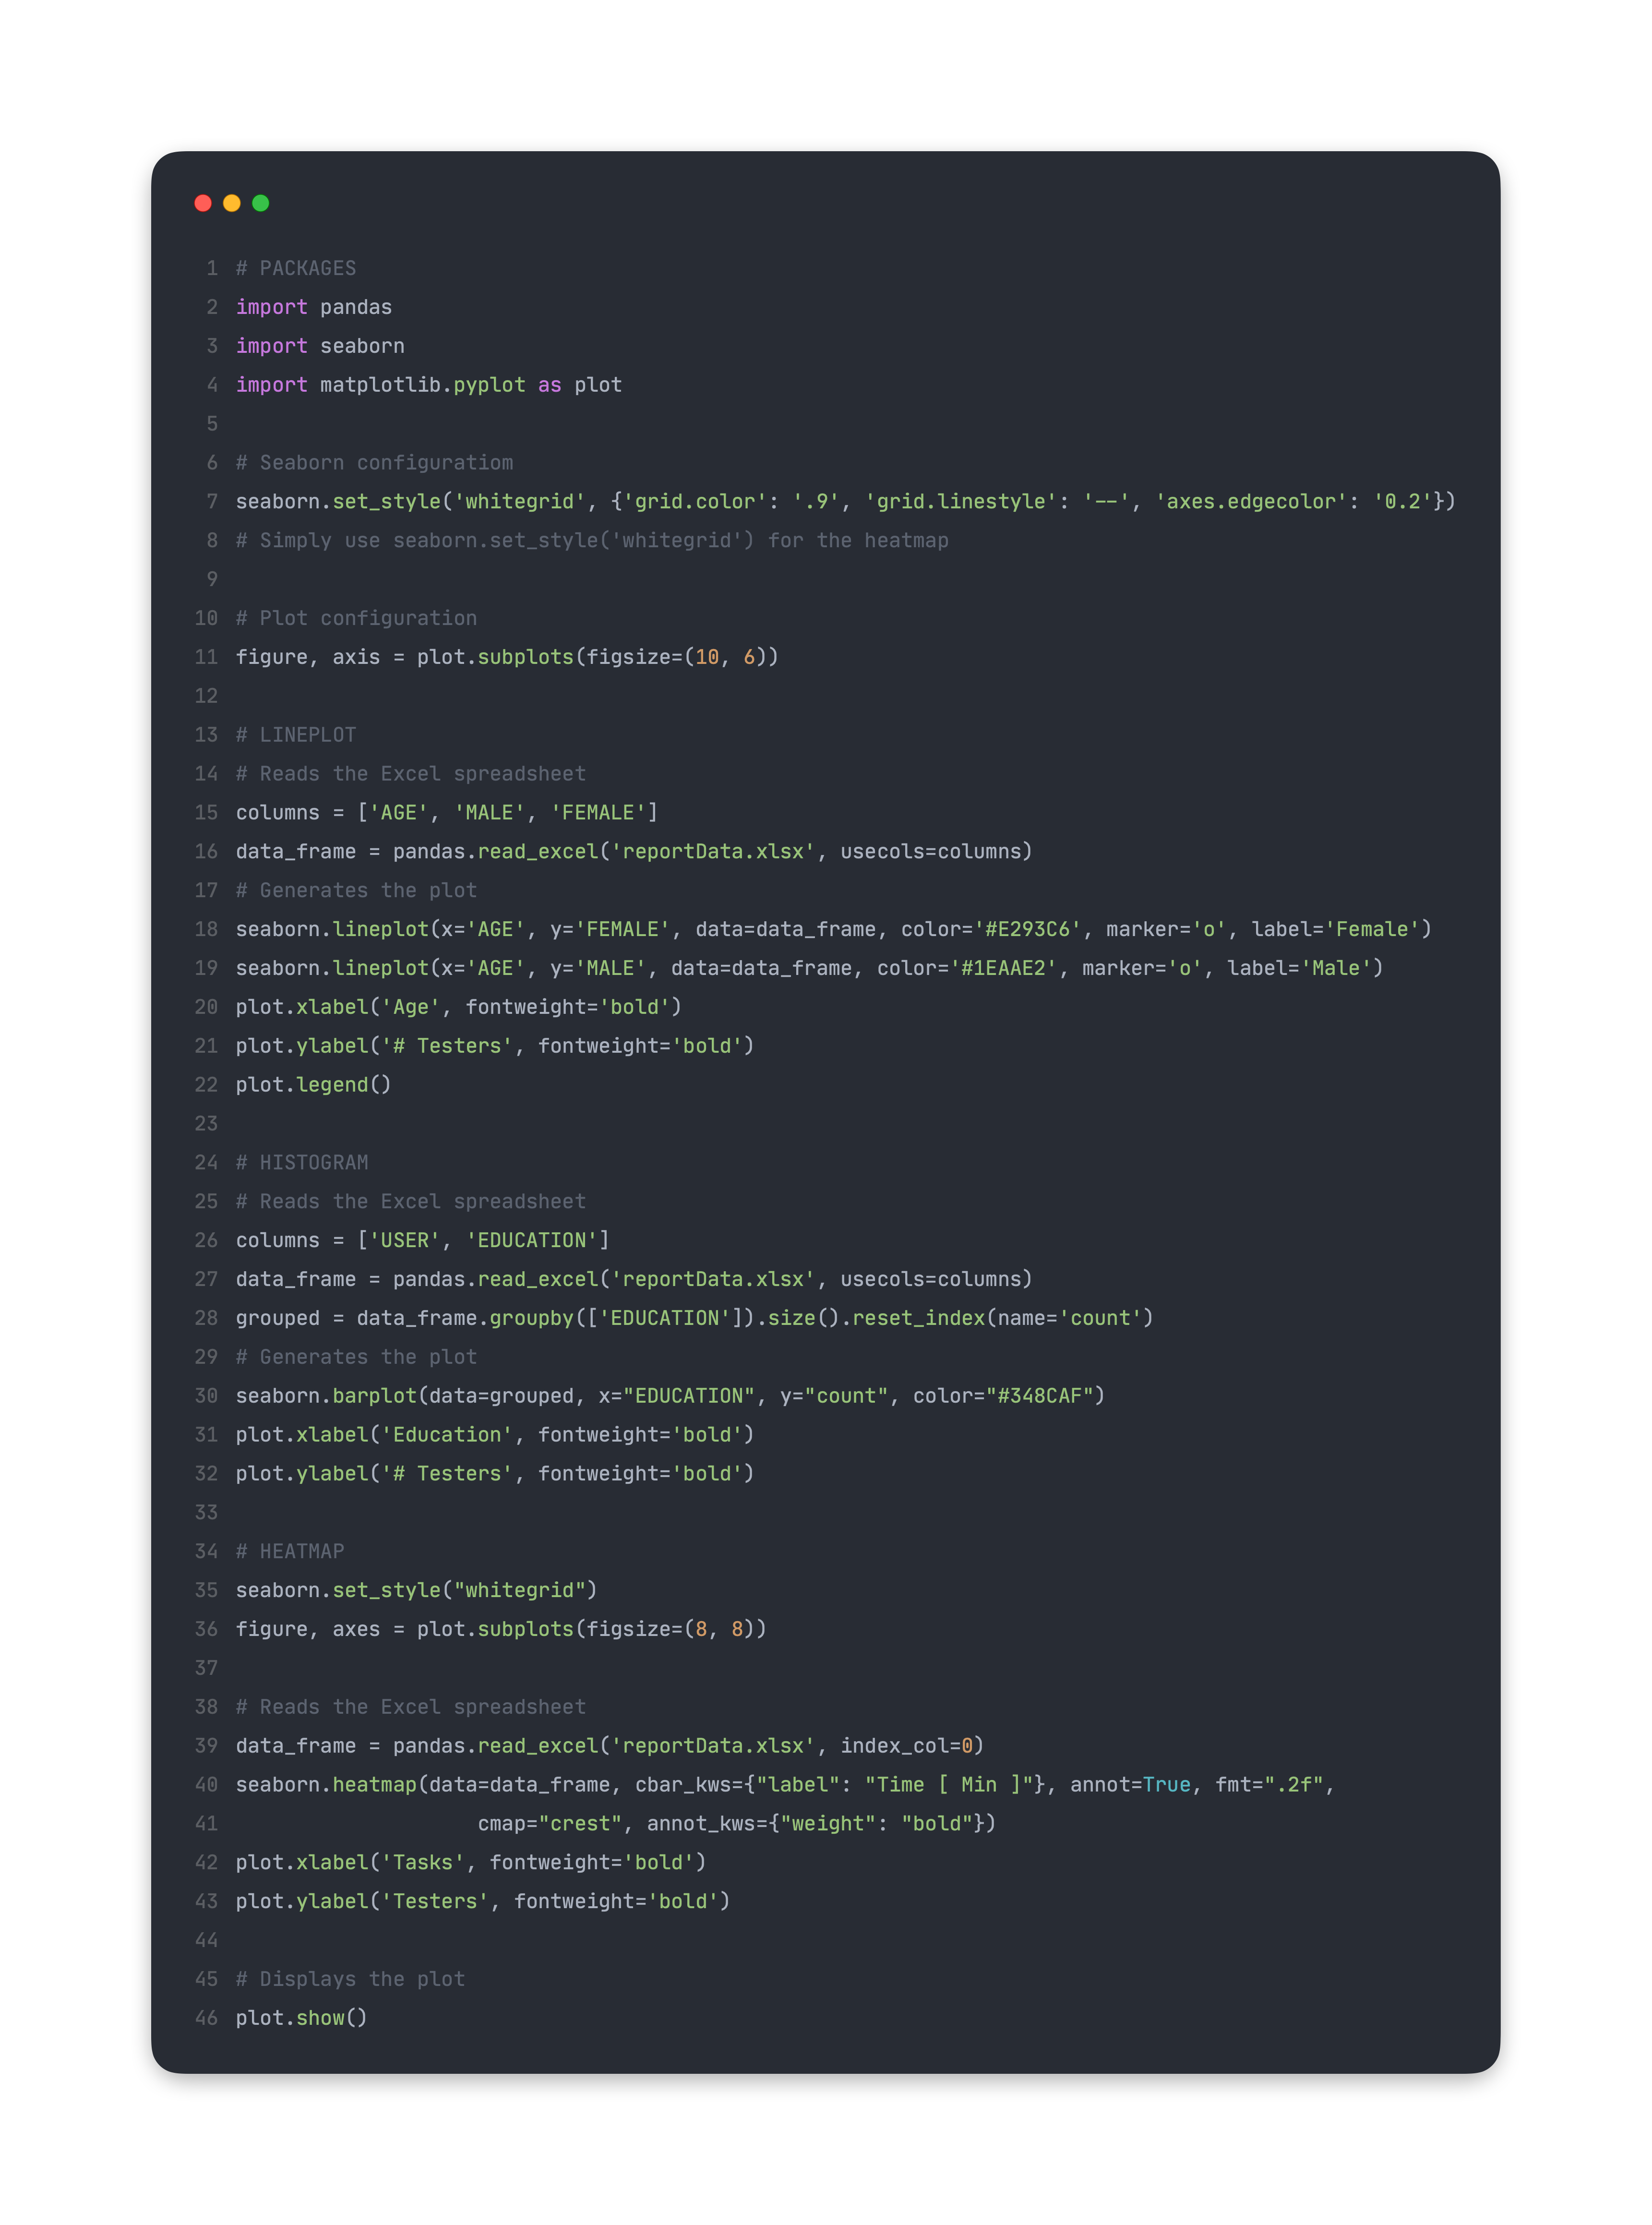
\includegraphics[scale=0.115]{Resources/Shared/pythonCode.png}
    \caption{Combined Python scripts for data plotting}
\end{figure}

\newpage

Figure (17) shows the age of the group of twenty-one users selected for the testing phase. 
Most of the users were between 23 and 25 years old, with the exception of three users who were over 25 years old, while the oldest user was 34 years old. 
It appears from this graph that the sample selected for testing was gender balanced, as it included 10 males and 11 females. 
  
\begin{figure}[htp!]
    \centering
    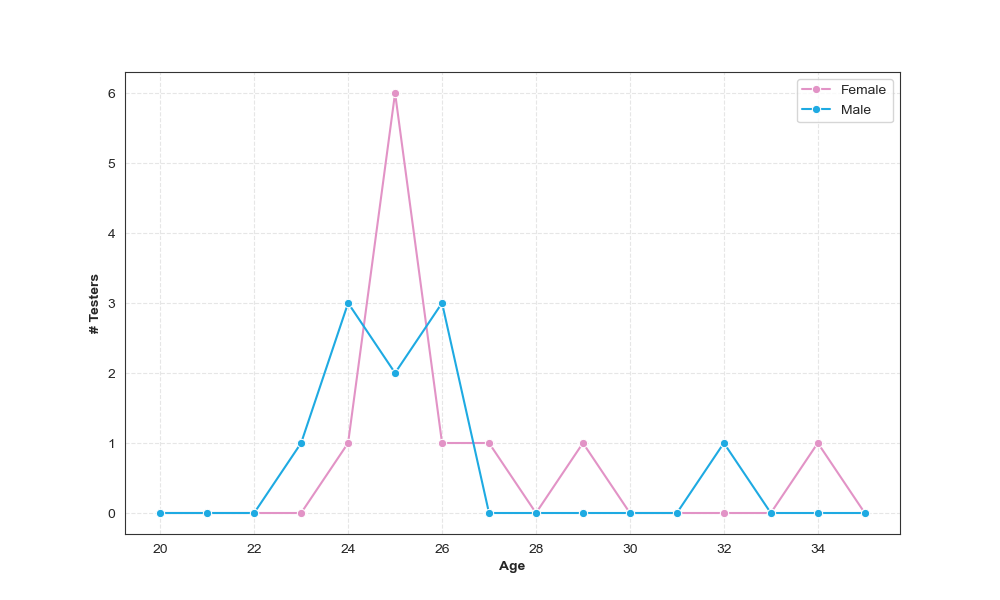
\includegraphics[scale=0.35]{Resources/Shared/agePlot.png}
    \caption{Age plot}
\end{figure}

Figure (18) shows the educational level of the test subjects. 
All users were or are in university education, albeit at different levels. 
Figure (18) shows the educational level of the test subjects. 
All users were or are in university education, albeit at different levels. 
Approximately 50\% of the users referred to themselves as students having or attending a master of science ( MSc. ) degree.
Following this, the most populous sample is that of a Bachelor of Science ( BSc. ) with no less than five members. 

\begin{figure}[htp!]
    \centering
    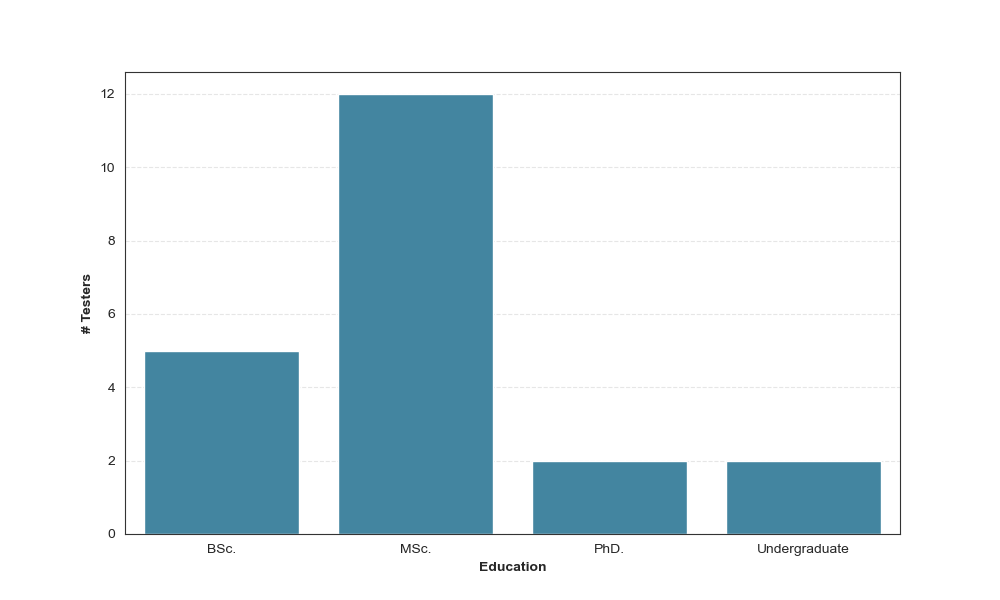
\includegraphics[scale=0.30]{Resources/Shared/educationPlot.png}
    \caption{Education level plot}
\end{figure}

\newpage
Finally, figure (19) represents a graph showing the time taken to complete each task by each user. 
From this plot, we can see that the majority of users were able to complete the assigned tasks quickly and profitably. 
This is immediately noticeable visually due to the predominance of the colour light green, which indicates completion times of less than two minutes. 
However, the heatmap also highlights the tasks that caused the most problems for users, highlighted by shades turning blue. 

\begin{figure}[htp!]
    \centering
    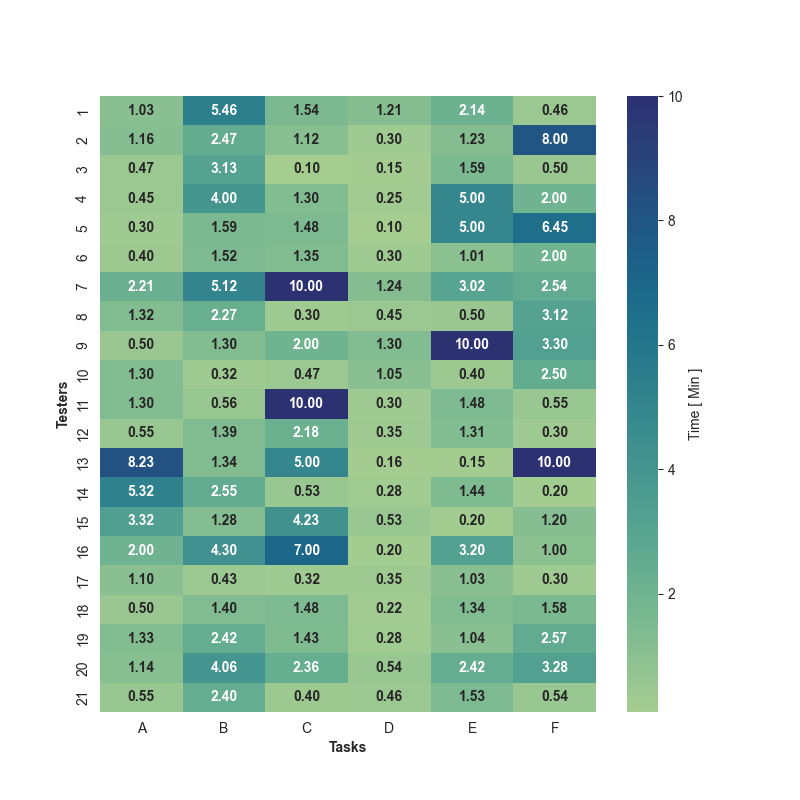
\includegraphics[scale=0.55]{Resources/Shared/taskstimePlot.png}
    \caption{Tasks completion time heatmap}
\end{figure}

\newpage
\subsection{Analysis}

Overall, we are satisfied with the results obtained during the testing phase. 
Most of the users managed to complete the assigned tasks below the time limits, however with task D being the only one where all users finished below the expected time.
Probably the most significant observation concerns the presence of outliers in task completion times. 
In tasks A, C, E and F, there were users who greatly exceeded the expected time threshold, even though most of their colleagues completed the task in a timely manner. 
This suggests that although the website appears to be well designed for a wide range of users, some improvements can and should be made so as not to discourage some users from using the site. 
This effect is most evident in task F where the two fastest users found the required information in 30 seconds, while the two slowest users took 8 minutes and 11 minutes. 
This suggests that there are some flaws in the design of the website. 
We believe that this discrepancy may be attributable to the different backgrounds of the users. 

Below are the most frequent comments received from users after the test procedure: 

\begin{itemize}
    \item Many testers experienced difficulties in navigating certain areas of the site, especially when trying to return to the homepage.
    \item Several users conveyed experiencing information overload while using the site.
    \item Users who utilized the site in Japanese and Chinese were dissatisfied with the translations provided.
\end{itemize}

These comments add more context to completion times.
Even though the vast majority of users managed to complete their tasks within the time limit, sentiment was not positive.
Users overall described some operations as frustrating and difficult, with navigation and information overload being the biggest pain points.
Taking action to improve these aspects of the site would therefore allow us to provide a better experience for users.
It's also interesting to note that users who chose to use the website's Japanese and Chinese language options were particularly dissatisfied with their experience.
Since UNICEF is an international organization, it is very important that it has multiple quality language options in order to extend accessibility and inclusiveness.
